\newpage

\section{Fourier Transforms of Periodic Functions and Local Solvability of Partial Differential Operators}

\subsection{Fourier transforms of periodic functions}
A function $f$ is periodic if
$$
f(x)=f(x+a)
$$
for some $a$ and for all $x$.

\begin{definition}
    [Periodic]
    $f \in \mathcal{D}^{\prime}$ is periodic of period $a$ if
$$
f(\phi)=f(\phi(\cdot+a))
$$
\end{definition}

Suppose $f$ is periodic, what can we say about $\widehat{f}$ ? Recall that for functions,
$$
\widehat{f}(\cdot+a)=e^{i a \cdot \xi} \hat{f}
$$
Using the periodic condition, write this as the multiplication
$$
\widehat{f} \cdot \left(1-e^{i a \xi}\right)=0
$$
Note that $1-e^{i a \xi} \neq 0$ unless $\xi=\frac{2 \pi n}{a}$. Then $\operatorname{supp} \widehat{f} \subseteq \frac{2 \pi n}{a} \mathbb{Z}$. As an analogy look at the condition $x f=0 \Longrightarrow f=c \delta_{0} ;$ here, we have zeros at many points. So we conclude that
$$
\widehat{f}=\sum_{n} c_{n} \delta_{\frac{2 \pi n}{a}}
$$

\begin{theorem}
The coefficients $c_n$ are the Fourier coefficients for $f$ in the interval $[0,a]$, and 
\[
    f(x) = \sum_n c_n e^{\frac{2\pi i}{a}nx}.
\]
\end{theorem}

Here, we have ignored the factors of $2\pi$.

\begin{remark}
    We can multiply $f$ by $e^{-\frac{2 \pi i}{a} m}$ and integrate from 0 to $a$ to get
    $$
    c_{n}=\int f(x) e^{-\frac{2 \pi i}{a} m x} .
    $$
\end{remark}

\begin{example}
    The simplest periodic distribution is
    $$
    f_{a}=\sum_{n} \delta_{n a}.
    $$
    Then
$$
\widehat{f}_{a}=\sum_{n} c_{n} \delta_{\frac{2 \pi}{a} n}
$$
If we write
$$
f_{a}\left(1-e^{\frac{2 \pi i x}{a}}\right)=0
$$
then we get
$$
\widehat{f}_{a}=\widehat{f}_{a}\left(\cdot+\frac{2 \pi}{a}\right) .
$$

Thus, all the $c_{n} \mathrm{~s}$ are the same. So
$$
\widehat{f}_{a}=c_{a} \sum_{n} \delta_{\frac{2 \pi n}{a}}=c_{a} f_{\frac{2 \pi}{a}}
$$
What is $c_{a} ?$ Apply this to a Schwarz function: $\widehat{f}(\phi)=f(\widehat{\phi})$ by definition, so
$$
c_{a} \sum_{n \in \mathbb{Z}} \phi\left(\frac{2 \pi n}{a}\right)=\sum_{m \in \mathbb{Z}} \widehat{\phi}(m a)
$$
This is called the \textbf{Poisson summation formula}.
Now what happens if we replace $\phi$ by $\phi e^{i x} \cdot \xi_{0}$ ? Then $\widehat{\phi}(\xi)$ becomes $\widehat{\phi}\left(\xi-\xi_{0}\right)$. The Poisson summation formula gives
$$
c_{a} \sum_{n} \phi\left(\frac{2 \pi n}{a}\right) e^{i \frac{2 \pi n}{a} \xi_{0}}=\sum \widehat{\phi}\left(m a-\xi_{0}\right)
$$
The dependence of $\xi_{0}$ on the left hand side is simple. Integrate to get
$$
\begin{aligned}
\underbrace{\int_{0}^{a} \sum_{n} \phi\left(\frac{2 \pi n}{a}\right) e^{i \frac{2 \pi n}{a} \xi_{0}} d \xi_{0}}_{=a c_{a} \phi(0)} &=\int_{0}^{a} \sum_{m} \widehat{\phi}\left(m a-\xi_{0}\right) d \xi_{0} \\
&=\int \widehat{\phi}(\xi) d \xi \\
&=\widehat{\phi}(1) \\
&=\phi\left(\frac{1}{\sqrt{2 \pi}} \delta_{0}\right)\\
&=\frac{1}{\sqrt{2\pi}} \phi(0)
\end{aligned}
$$
Accounting for the constants we ignored before, we get
$$
c_{a}=\frac{1}{2 \pi a} .
$$
\end{example}

\begin{remark}
    We can use the Poisson summation formula to compute all sorts of series. Recall that $\mathcal{F}\left(\frac{1}{1+x}\right)=c e^{-|\xi|}$ (perhaps omitting constants). Choose $a=2 \pi$. The Poisson summation formula tells us that
    $$
    \sum_{m \in \mathbb{Z}} \frac{1}{n^{2}+1}=\sum_{m} e^{-2 \pi|m|}=\frac{2}{1-e^{2 \pi}}-1
    $$
    where we have ignored the constants.
\end{remark}

\subsection{Local solvability of partial differential operator}
Let $P(D)$ be our partial differential operator with constant coefficients.

\begin{definition}
    [Solvable]
    $P(D)$ is solvable if for each $f$, the equation $P(D)u=f$ admits at least one solution.
\end{definition}
If $f \in \mathcal{D}^{\prime}$, then $u \in \mathcal{D}^{\prime} .$ If $f \in \mathcal{S}$, then $u \in \mathcal{S} .$ In general, the regularity of $f$ and $u$ will be related, so when we say $P(D)$ is solvable, we specify a class of functions $f$.

\begin{definition}
[Locally solvable I]
$P(D)$ is locally solvable if for each $f\in \cE'$, there exists a solution $u\in \cD'$ in a neighborhood of the support of $f$.
\end{definition}
If $u \in \mathcal{E}^{\prime}$, then $P(\xi) \widehat{u}(\xi)=\widehat{f}(\xi)$ for $\xi \in \mathbb{C}^{n} .$ Here is a narrower version, which we may regard as the "real definition" of local solvability:

\begin{definition}
    [Locally solvable II]
     $P(D)$ is locally solvable if for each $x_{0}$, there is an $\varepsilon>0$ such that if $\operatorname{supp} f \subseteq B\left(x_{0}, \varepsilon\right)$, then a solution exists.
\end{definition}
For today, we will deal with the first, more relaxed definition.

\begin{theorem}
    Every constant coefficient partial differential operator is locally solvable (in the relaxed sense).
\end{theorem}
\begin{proof}
    Suppose $f$ is supported in $B \subseteq[0,2 \pi]^{n} .$ Take $\widetilde{f}$ to be the periodic extension of $f$, and look for a periodic solution $\widetilde{u}$ to $P(D) \widehat{u}=\widetilde{f}$.
    \begin{figure}[H]
        \centering
        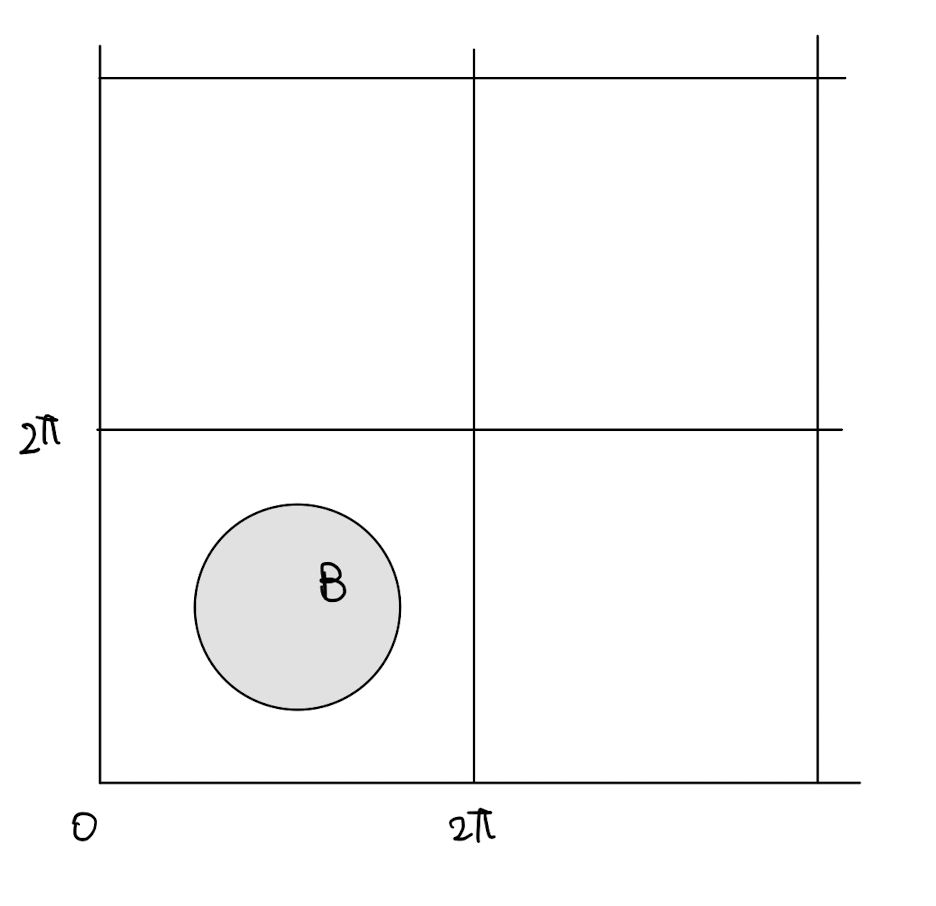
\includegraphics[width=0.5\textwidth]{pics/21-1.png}
    \end{figure}
    What does this periodization do? Originally, $P(D) u=f$ gives $P(\xi) \widehat{u}=\widehat{f}$, so $\widehat{u}=\frac{1}{P(\xi)} \widehat{f}$ However, this has issues because $P(\xi)$ can have issues. In the periodic case, we know
$$
\begin{aligned}
&\widehat{\widetilde{f}}(\xi)=\sum_{m \in \mathbb{Z}^{n}} f_{m} \delta_{m} \\
&\widehat{\widetilde{u}}(\xi)=\sum_{m \in \mathbb{Z}} u_{m} \delta_{m}
\end{aligned}
$$

The advantage is that we only $P(m) \neq 0$ on lattice points $m \in \mathbb{Z}^{n}$. However, the Fourier transform is defined for temperate distributions, so we need about on $\frac{f_{m}}{P(m)}$. More precisely, we need a bound
$$
|P(m)| \geq(1+|m|)^{-N}
$$
What if $P$ has zeroes on the lattice points? Make the change of notation $f \mapsto f e^{i x \cdot \xi}=g$ so $u \mapsto u e^{i x \xi}=v$. We can ask this question for the phase-shifted variables. To study our equation, we need to expand
$$
P(D) u=P(D)\left(v e^{-i x \cdot \xi}\right)
$$
To use the Leibniz rule, note that,
$$
\begin{aligned}
D_{j}\left(v e^{-i x \xi}\right) &=D_j v e^{-i x \xi}+v D_{j} e^{-i x ; \xi} \\
&=e^{-i x \cdot \xi}\left(D_{j} v-v \xi_{j}\right)\\
& = e^{-x\cdot \xi}(D_j -\xi_j)v,
\end{aligned}
$$
We can write this as $e^{i x \cdot \xi} D_{j} e^{-i x \xi}=D_{j}-\xi_{j}$, which we may think of as a conjugation. Referring to our equation, we get
\[
\begin{aligned}
    P(D) u &=P(D)(ve^{-ix\cdot \xi})\\
    &=e^{-i x \cdot \xi} p(D-\xi) v \\
    &=f
    \end{aligned}
\]
which tells us that we have replaced $P(D) u=f$ with
$$
P(D-\xi) v=g
$$
So we only need to solve the new periodic problem is to define
$$
v_{m}=\frac{g_{m}}{P(m-\xi)}, \quad m \in \mathbb{Z}
$$
Now we only need to find some $\xi \in[0,1]^{n}$ such that
$$
|P(m-\xi)| \geq(1+|m|)^{-N} \quad \forall m
$$
The following lemma tells us we can find such a $\xi$.

\begin{lemma}
    If $\delta$ is small enough, then
$$
\int \frac{1}{(P(\eta))^{\delta}} \frac{1}{(1+|\eta|)^{N}} d \eta<\infty .
$$
\end{lemma}
\begin{proof}
     In 1 dimension, use partial fractions. Then reduce any number of dimensions to the 1-dimensional case.
    \qed 
\end{proof}

\vspace{2em}
How does this help us? Write $\eta=m+\xi$ with $m \in \mathbb{Z}^{n}$ and $\xi \in[0,1]^{n}$. Then
$$
\int_{\xi} \sum_{m} \frac{1}{P(m-\xi)^{\delta}} \frac{1}{(1+|m|)^{N}} d \xi<\infty
$$
So for almost every $\xi$,
$$
\sum_{m} \frac{1}{|P(m-\xi)|^{\delta}} \frac{1}{(1+|m|)^{N}}=M<\infty
$$
This tells us that
$$
|P(m-\xi)| \geq M^{-1 / d}(1+|m|)^{-N / \delta}
$$
which is exactly the relation we want to have.
\qed 
\end{proof}